\documentclass[aps,prd,amsmath,showpacs,amssymb,superscriptaddress,nofootinbib,longbibliography,eqsecnum,preprintnumbers]{revtex4-1}
\usepackage{graphicx}
\usepackage{bm}
\usepackage{amssymb,amsmath}
\usepackage{mathrsfs}
\usepackage{braket} 
\usepackage{latexsym}
\usepackage{color}
\usepackage{float}
\usepackage[normalem]{ulem} 
\usepackage{dcolumn}
\usepackage[colorlinks=true,citecolor=blue,urlcolor=blue]{hyperref}
\usepackage[usenames,dvipsnames]{xcolor}

\allowdisplaybreaks

\newcommand{\Sph}{{}_{-2}S_{\ell m n_{\pm}}}
\newcommand{\Ys}{{}_{-2}Y_{\ell m}}
\newcommand{\mul}{{\ell m n_{\pm}}}
\newcommand{\Caltech}{\affiliation{Theoretical Astrophysics 350-17, California Institute of Technology, Pasadena, CA 91125}}
\newcommand{\CITA}{\affiliation{Canadian Institute for Theoretical Astrophysics, 60 St. George Street, Toronto, ON, M5S 3H8 Canada}}
\newcommand{\zach}[1]{\textcolor{ForestGreen}{#1}}
\newcommand{\acs}{\alpha_{\rm CS}}
\newcommand{\bcs}{\beta_{\rm CS}}
\newcommand{\Ssh}{S_{\rm shot}}
\newcommand{\Techo}{T_{\rm echo}}

\begin{document}
\title{Measuring the Angular Emission of the Ringdown}
%\author{Zachary Mark} \Caltech
\begin{abstract}
We design a test to determine if the angular emission during the ringdown of a Kerr black hole is described by spheroidal harmonics as is predicted by the black hole perturbation theory. 
\end{abstract}
\maketitle
\tableofcontents

\section{Spherical Harmonic Decomposition}

Quasi-circular Binary black hole waveforms depend on 15 parameters: the BH masses $m_1$ and $m_2$ (We will often parameterize these masses with the total mass $M=m_1+m_2$ and the symmetric mass ratio $\nu =m_1m_2/M^2$); the BH spins $\vec s_i$; two angles localizing the source, i.e. the declination $\delta$, and the right ascension $\alpha$; three angles specifying the direction of the source, i.e. the inclination of the orbit relative to the line of sight $\iota$, the polarization angle $\psi$ (these angles are defined in appendix \ref{sec:coor}), and a phase $\phi_*$ that defines the orientation of the binary around its angular momentum (for example, this phase might be defined as the phase at coelescence $\phi_c$); the arrival time $t_*$; and the proper distance $d$ to the source. We will collectively refer to these ``GR'' parameters as $\lambda^i$ and use i as an index that runs of over the GR parameters. 

First consider an observer in the local wave frame where redshift can be ignored. In the wave frame\footnote{The wave frame is defined in appendix \ref{sec:coor}}, the waveform can be decomposed in spin weighted spherical harmonics
\begin{align}
\tilde H(f;\nu,M,\vec s_1,\vec s_2, d,\iota,t_*,\phi_*)
&\equiv \tilde h_+-i\tilde h_\times \nonumber \\
&=\frac{GM}{c^2d}\sum_{\ell =2}^\infty \sum_{m=-\ell}^\ell \tilde h_{\ell m}\left(f;M, \nu, s_1,s_2\right)\Ys(\iota, 0)e^{-2\pi i f t_* -im\phi_*} \label{eq:dec}
\end{align}
For observers at cosmological distances, we must include the effect of redshift .To include the effect of redshift all parameters with length dimension $\mathcal{L}^p$ should be multiplied by $(1+z)^p$, i.e. the mass $M\to M_z=(1+z)M$ becomes the redshifted mass (and the M on the RHS is the mass measured in the rest frame) and the proper distance $d\to d_L=d(1+z)^p$ becomes the luminosity distance (and the d on the RHS is the proper distance). Note that the frequency is not redshifted with this prescription \cite{Berti:2005ys,Flanagan:1997sx}.

As is discussed in appendix \ref{sec:coor}, we orient our source frame so that observer has an azimuthal angle of of $0$.
The spherical harmonic modes $h_{\ell m}$ only depend on the masses and the spin parameters. The factor of $e^{-2\pi if t_*}$ is the frequency domain version of a shifted start time\footnote{using the convention $\tilde H= \int dt e^{-2\pi i ft}H(t)$.}. The dependence on $\phi_*$ comes from the fact that if we rotate the binary by $\phi_*$ in the azimuthal direction, we get the same waveform as before with $\phi \to \phi-\phi_*$. Since the spin-weight spherical harmonics $\propto e^{im \phi}$, we can parameterize the waveforms of rotated binaries with the factor $e^{-im\phi_*}$.

Later on if we consider $N_O$ observations, we will label each observation by a lower case latin letter enclosed in parenthesis, i.e (k). Each observation will have different parameters and we will use the following (redundant) notation: subscripted indices $i_{(k)}$ label the parameters for the kth observation $\lambda^{(k)}_{i_{(k)}}$.

\section{The angular emission of the ringdown}

A binary black hole (BBH) waveform   consists of an inspiral, a merger, and a ringdown. In the frequency domain, one can define the ringdown part of the waveform as the high frequency component 
\begin{align}
\tilde H&=\int dt e^{-2\pi i f t} H(t) 
\nonumber \\
&=
\begin{cases}
\tilde H^{\rm In}& f<f_c \\
\tilde H_{\rm ring}& f>f_c.
\end{cases}
\end{align}
Here $f_c$ is a cut-off frequency, which is approximately the ISCO frequency of the final Kerr black holes as in (\zach{ZM: cite golden binary paper.})
Here $\tilde H ^{\rm In}$ is the low-frequency portion waveform and is accurately predicited by both post-newtonian theory or numerical relativity. Both the inspiral and the ringdown have spherical harmonic decompositions. 
%We will refer to the spherical harmonic modes during the ringdown as $\alpha_{\ell m}$, i.e $\tilde h^{\rm ring}_{\ell m}=\alpha_{\ell m}$. 

At all times general relativity predicts a unique relationship between the spherical harmonic modes $h_{\ell m}$ which encodes the angular emission pattern of the radiation. Most interesting is the angular emission pattern during the ringdown, which is governed by general relativity in the least-tested strong field regime.

In the time domain, the ringdown portion of the waveform starts at approximately $t\approx t_R$, where $t_R$ is chosen to be slightly after the peak of the waveform. During the ringdown, general relativity predicts that the waveform is well-approximated by a QNM sum\footnote{Note that I am following London et. al. and using the unconventional sign convention $e^{i\omega_\mul}$ rather than $e^{-i\omega_\mul}$}, i.e in the wave frame \footnote{The wave frame is defined in appendix \ref{sec:coor}. Note that we have made the assumption that the observer is located at an azimuthal angle of 0 relative to the source and that this assumption does not fix the orientation of the source because we have the freedom to change the coalescence phase. Also note that $\psi_4= \ddot H$.}
\begin{align}
H_{\rm ring}^{GR}=h_+-ih_\times=\frac{GM}{dc^2}\sum_{\ell m n_{\pm}}B_{\ell m n\pm}e^{i\omega_{\ell m n_{\pm}}(t-t_*-t_R)}\Sph(\iota,0)\theta(t-t_*-t_R)e^{-im\phi_*},
\end{align}
%where $\tau =t-t_*-t_R$

The QNM frequencies $\omega_\mul$ and angular functions $\Sph(\theta, \phi)$, which are known as spin-weighted spheroidal harmonics, can be calculated from the Teukolsky equation. They are indexed by spheroidal harmonic multipoles $\ell$ and m and an overtone $n_\pm$. The subscript $\pm$ refers to the co-rotating and counter rotating QNM frequencies. The complex amplitudes $B_\mul$ are difficult to predict from first principals but have been obtained by fitting numerical relativity waveforms. London et al. \cite{London:2014cma} have provided fits as functions of symmetric mass ratio $\nu=\frac{m_1m_2}{(m_1+m_2)^2}$ for the $A_{\ell m n_\pm}=-\omega_{\ell mn\pm}^2sM_{\rm remnant}B_{\ell mn \pm}$. For the $(\ell m n) =220+$ mode from Eq. 2\footnote{Recall with London's convention (which we follow here as well) that uses $e^{i\omega_{220}t}$ for the time dependence of each ringdown mode, the QNM's have a positive imaginary part. Also not London appears to have oriented his binary so $A_{220+}/\omega_{220+}^2$ is real}
%\footnote{Note that I have used a slightly different convention than london, i.e. $A_{\ell m n}^{rm here}=A_{\ell m n}^{rm London}$},
\begin{align}
A_{220+}=\omega_{220+}^2\left(0.9252 \nu +0.1323\nu^2 \right)
\label{eq:A220}
\end{align}
To use this formula, we must calculate $\omega_{220+}$ with the final black hole mass $M_f(m_1,m_2)$ and dimensionless spin $j_f(m_1,m_2)$, which can be obtained with fitting formula in Appendix C of London, see eq. C2\footnote{In these equations, London uses units where $m_1+m_2 =1$}.

A measurement of the $h_{\ell m}$ is equivalent to a measurement of the spheroidal harmonics.
If we assume a single mode ringdown, dominated by the $\mul=220_+$ mode, the ringdown waveform can be re-expanded in spin weight spherical harmonics $\Ys$
\begin{align}
H_{\rm ring}=\frac{GM}{dc^2}\sum_{\ell}B_{\ell m n \pm}e^{i\omega_{220+}(t-t_*-t_R)}\sigma_{220_+\ell }{}_{-2}Y_{\ell 2}(\iota,0) \theta(t-t_*-t_R)e^{-im\phi_*},
\end{align}
where we have used the expansion of the spheroidal harmonics\footnote{Note that Berti et al. \cite{Berti:2014fga} have calculated $u_{m\ell \ell'n}=\sigma_{\ell'mn\ell}^*$. We use Berti's data in our calculations.}
\begin{align}
&\Sph(\theta, \phi)=\sum_l'\sigma_{\ell m n_{\pm} \ell'}{}_{-2}Y_{\ell'm}(\theta,\phi) \nonumber \\
&\sigma_{\ell m n_\pm \ell'}=\braket{{}_{-2}Y_{\ell' m}|\Sph}\equiv \int d\Omega {}_{-2}Y^*_{\ell ' m}\Sph(\theta,\phi)
\end{align}
Hence we see that general relativity predicts that\footnote{We set $t_*=0$ to be consistent with the convention in Eq.~\eqref{eq:dec}} 
\begin{align}
h_{\ell m}(t)=
\begin{cases}
0 & m\neq 2 \\
B_{\ell m n\pm}\sigma_{220_+\ell }e^{i\omega_{220+}(t-t_R)}\theta(t-t_R)
\end{cases}
\end{align}

To test the angular emission pattern during ringdown, we write a generic, potentiall non-GR ringdown as
\begin{align}
h_{\ell m}(t)=\alpha_{\ell m}e^{i\omega (t-t_R)} \theta(t-t_R) \label{eq:genr}
\end{align}
%To test the angular emission pattern during ringdown, we write a generic, potentiall non-GR ringdown as 
%\begin{align}
%H_{\rm ring}=\frac{GM}{dc^2}\sum_{\ell m}\alpha_{\ell m}e^{i\omega \tau}\Ys(\iota,0). \label{eq:genring}
%\end{align}
or in the frequency domain
\begin{align}
\tilde h_{\ell m}(f)=\frac{i\alpha_{\ell m}}{\omega -2\pi f}e^{-2\pi i ft_R}
\end{align}
Note that the generic ringdown is parameterized by the complex parameters ${\theta_A}=\{\omega,\{\alpha_{\ell m}\}\}$. We will use upper case latin indices to run over these parameters characterizing the deviation from GR.

Our test will assume that the true theory predicts the same inspiral waveform as GR. This assumption is equivalent to assuming that the true theory agrees with GR in the post-newtonian, weak field regime and has some backing in experiment. Hence we will incorporate the modified ringdown by using the GR prediction for $h_{\ell m}$ during the inspiral and the generic Eq.~\eqref{eq:genr} for $h_{\ell m}$ during the inspiral.
% Hence, we will incorporate the modified ringdown in the waveform by writing the complete frequency domain waveform as a pure ringdown at high frequencies and an inspiral waveform at low frequncies (also see (\zach{ZM:cite waveform split test and others}))
% \begin{align}
% \tilde H&=\int dt e^{-2\pi i f t} H(t) 
% \nonumber \\
% &=
% \begin{cases}
% \tilde H^{GR}& f<f_c \\
% \tilde H_{\rm ring}& f>f_c.
% \end{cases}
% \end{align}
% Here $\tilde H ^{\rm GR}$ is the low-frequency portion waveform as predicted by GR and in practice in can be replaced with either a numerical relativity waveform or a Post-Newtonian waveform. Explicitly The fourier transform $H_{\rm ring}$ is
% \begin{align}
% \tilde H_{\rm ring}(f)=
% \frac{-1}{d}\sum_{\ell m} \frac{i\alpha_{\ell m}}{2\pi f-\omega}e^{-2\pi if (t_R+t_*)}\Ys(\iota,0).
% \end{align}
% We choose the cut-off frequency $f_c$ is be ... as in ...

\section{Strain at each detector}

We now imagine that we have $N_D$ detectors detecting each event. We label each detector with a capitol latin letter enclosed in parenthesis, i.e. (A). Suppose an event produces the TT metric perturbation at the center of the earth
\begin{align}
\tilde h_{ij}(f)=\tilde h_+(f;\theta_A,d,t_*,\iota)e_{ij}^+(\delta,\alpha,\psi) +\tilde h_\times(f;\theta_A,d,t_*,\iota)e_{ij}^\times(\delta,\alpha,\psi).
\end{align}
Here $e^+_{ij}$ and and $e^\times_{ij}$ are the wave frame polarization tensors
\begin{align}
e^+_{ij}(\delta,\alpha,\psi)&=(\vec e_X)_i(\vec e_X)_j-(\vec e_Y)_i(\vec e_Y)_j), \nonumber \\
e^\times_{ij}(\delta,\alpha,\psi)&=(\vec e_X)_i(\vec e_Y)_j+(\vec e_Y)_i(\vec e_Y)_j)
\end{align}
with $\vec e_X$ and $\vec e_Y$ given Eq.~\eqref{eq:wavebasis} in appendix \ref{sec:coor}.

Each detector is characterized by a detector tensor $D_{(A)}^{ij}$ and a location $\vec r_{(A)}$ (defined in the earth-centered coordinate system of appendix \ref{sec:coor}) and the values for existing detectors are given in tables A1-A3 of \cite{Creighton:2011zz}. For an interferometer with arm vectors $\vec p$ and $\vec q$,
\begin{align}
D^{ij}=\frac{1}{2}\left [\hat p^i\hat p^jD(\hat p \cdot \hat n, f||p||/c)-\hat q^i\hat q^jD(\hat q \cdot \hat n, f||q||/c)\right],
\end{align}
\begin{align}
D(\mu,x)=\frac{1}{2}e^{2\pi ix}\left[e^{i\pi x(1-\mu)}sinc(\pi x(1+\mu))+e^{-i\pi x(1+\mu)}sinc(\pi x(1-\mu))\right]
\end{align}
Here $\hat n= -[\sin\theta \cos\phi \hat x'+\sin\theta \sin\phi \hat y'+\cos\theta \hat z']$, with $\theta =\pi/2-\delta$ and $\phi=\alpha -\text{(Greenwich Mean Sidereal Time)}$ being the source's angular position in the earth frame;and $\{\hat x',\hat y',\hat z'\}$ being the cartesian basis in the earth frame, points in the direction of the wave propagation.
In the limit the wavelength\footnote{\zach{ZM: note the typo in Creighton, who says $D\to 1$ in the long wavelength limit.}} of the GW's is large with respect to the length of the interferometer arms, $D\to 1$ and $D^{ij}$ becomes independent of frequency and source direction.

The strain measured at the $(A)$ the detector is
\begin{align}
\tilde h_{(A)}=e^{-2\pi i f \tau}D_{(A)}^{ij}\tilde h_{ij}(f)=e^{-2\pi i f \tau}\left[G^{(A)}_+\tilde h_++\tilde G^{(A)}_\times h_\times\right],
\end{align}
where $\tau_{(A)} \equiv \vec r_{(A)}\cdot \hat n/c$ the detector pattern response functions have been defined as
\begin{align}
G^{(A)}_{+,\times}(\delta, \alpha ,\psi)=D_{(A)}^{ij}e^{+,\times}_{ij}
\end{align}

We now specialize to interferometric detectors with arms at a right angle. Furthermore, we specialize to the long wavelength limit when the detector tensor becomes independent of the frequency and the wave-propagation direction (i.e source location) $D^{ij}=\frac{1}{2}\left[\hat p^i \hat p^j-\hat q^i \hat q^j\right]$.
In this limit, when $\hat p= [1,0,0]$ and $\hat q=[0,1,0]$
\begin{align}
G^{(A)}_+(\alpha,\delta,\psi)&=
\frac{1}{2}(1+\cos^2\theta)\cos (2\phi_{(A)})\cos (2\psi)-\cos \theta \sin (2\phi_{(A)})\sin (2\psi) \nonumber \\
G^{(A)}_\times &=-\frac{1}{2}(1+\cos^2\theta)\cos (2\phi_{(A)})\sin(2\psi)-\cos \theta \sin(2\phi_{(A)})\cos (2\psi),
\end{align}
where $\theta =\pi/2 -\delta$ and $\phi_{(A)}=\alpha-GMST(A)$, and we can write the time domain strain measured by the detector as
\begin{align}
h_{(A)}(t)&=\Re\left[(G^{(A)}_+-iG^{(A)}_\times)H(t-\tau )\right] \\
&=\Re\left[ (G_+^{(A)}-iG_\times^{(A)})\frac{GM}{dc^2}\sum_{\ell =2}^\infty\sum_{m=-\ell}^{\ell}h_{\ell m}([t-t_*-\tau_{(A)}]/M)\Ys(\iota,0)e^{-im\phi_*}\right]
\\
&=\frac{GM}{2dc^2}\sum_{\ell =2}^\infty\sum_{m=-\ell}^{\ell} \nonumber \\
&\left[(G^{(A)}_+-iG^{(A)}_\times)h_{\ell m}([t-t_*-\tau_{(A)}]/M)\Ys(\iota,0)e^{-im\phi_*} 
+(G^{(A)}_++iG^{(A)}_\times)h_{\ell m}^*([t-t_*-\tau_{(A)}]/M)\Ys^*(\iota,0)e^{im\phi_*}\right]
%\\
%&=\frac{GM}{2dc^2}\sum_{\ell =2}^\infty\sum_{m=-\ell}^{\ell}\Ys(\iota,0)e^{-im\phi_*}\left[(G^{(A)}_+-iG^{(A)}_\times)h_{\ell m}([t-t_*-\tau_{(A)}]/M)+(-1)^m(G^{(A)}_++iG^{(A)}_\times)h_{\ell -m}^*([t-t_*-\tau_{(A)}]/M)\right],
%\label{eq:restrain}
\end{align}
Also note that ${}_{-2}Y_{\ell m}^*(\theta ,\phi)=(-1)^m{}_{-2}Y_{\ell -m}(\pi-\theta ,\phi)$.

To get the frequency domain version of the strain in terms of the spherical harmonic modes, it is useful to note that the fourier transform of the complex conjugate is the complex conjugate of the fourier transform evaluated at $-f$, i.e
\begin{align}
\mathcal{FT}[g^*(t)&=\mathcal{FT}[g_R(t)-ig_I(t)]
\nonumber \\
&=\tilde  g_R(f) -i\tilde g_I(f) \nonumber \\
&=(\tilde g_R(-f))^*-i(\tilde g_I(-f))^* \nonumber \\
&=\tilde g(-f)^*.
\end{align}
Hence 
\begin{align}
\tilde h_{(A)}(f)&=\frac{GM}{2dc^2}\sum_{\ell =2}^\infty\sum_{m=-\ell}^{\ell}e^{-2\pi i f(t_*+\tau_{(A)})} \nonumber \\
&\left[(G^{(A)}_+-iG^{(A)}_\times)\tilde h_{\ell m}(Mf)\Ys(\iota,0)e^{-im\phi_*}+(G^{(A)}_++iG^{(A)}_\times)\tilde h_{\ell m}^*(-Mf)\Ys^*(\iota,0)e^{im\phi_*}\right] \label{eq:hsph1}
%\\
%&=\frac{GM}{2dc^2}\sum_{\ell =2}^\infty\sum_{m=-\ell}^{\ell}\Ys(\iota,0)e^{-im\phi_*}e^{-2\pi i f(t_*+\tau_{(A)})}
%\left[(G^{(A)}_+-iG^{(A)}_\times)\tilde h_{\ell m}(Mf)+(-1)^m(G^{(A)}_++iG^{(A)}_\times)\tilde h_{\ell -m}^*(-Mf)\right] \label{eq:hsph}
\end{align}

%In practice, when we model waveforms we will truncate the number of modes that we use and Eq.~\eqref{eq:hsph1} may be more useful than Eq.~\eqref{eq:hsph}.

% It is convenient to write the TT gauge metric perturbation $h_{ij}$ with it's value referred to the center of the earth in the wave frame. The wave frame is shown in figure...

% which produces a TT metric perturbation 
% \begin{align}
% h_{ij}(t)=h_+(t)e^+_{ij}(\delta,\alpha,\psi)+ h_\times(t)e^+_{ij}(\delta,\alpha,\psi)
% \end{align}
% at the center of the earth. Here we have decomposed $h_{ij}$ into the ``wave frame'' polarization tensors $e^+_{ij}(\delta,\alpha,\psi)$ and $e^\times_{ij}(\delta,\alpha,\psi)$ which depend on the location of the source characterized by $\delta$ and $\alpha$ aand 

% and each detector measures a strain $h^{(A)}=D_{{(A)}}^{ij}h_{ij}$, where $D_{(A)}^{ij}$ is the detector tensor for the $(A)$th detector, $h_{ij}$ are the spatial components of the metric perturbation, and in this context i an j are spatial indices, not indices labeling the parameters. We label each detector with capitol latin indices surrounded by parentheses. In general the detector tensor depends on the direction to the source. However, for interferometers in the long wavelength limit
% \begin{align}
% D_{(A)}^{ij}=\frac{1}{2}(\hat p_{(A)}^i\hat p_{(A)}^j-\hat q_{(A)}^i\hat q_{(A)}^j),
% \end{align}
% where $\hat p_{(A)}$ and $\hat q_{(A)}$ are unit vector directed along the arms of the $(A)$th interferometer. Expressing $h_{ij}=e^+_{ij}(\delta,\alpha,\psi)$

\section{Fisher Matrix}

Our goal is to estimate how well we can measure the parameters $\alpha_{\ell m}$ given $N_O$ observations with $N_D$ detectors. Each observation has $15$ GR parameters $\lambda^{(k)}_{i_{(k)}}$ and there are $L=2+2\sum_{\ell= 0}^{\ell_\text{max}}(2\ell+1)$ real parameters in $\{\theta_A\}=\{\omega,\{\alpha_{\ell m}\}\}$, where $
\ell_{\text{max}}$ is the largest $\ell$ that we include in the ringdown spherical harmonic sum. Hence there are $15N_O+L$ parameters in the problem.

Collectively, we will refer to all of the parameters as $\{P_\alpha\}=\{\theta_A\}\bigcup_{(k)}\{\lambda^{(k)}_{i_{(k)}}\}$, where we use greek indices to act as super indices running over all $15N_0+L$ parameters.
The effect of a measurement on our knowledge of the parameters is quantified by the likelihood function $\mathcal{L}(P_\alpha)$, which gives the probability of seeing the observed data given the parameters have the values $P_\alpha$.

Suppose the parameters have a the true values $\bar P_\alpha$ \zach{(ZM:Does this statement contradict a Bayesian framework)}. The maximum likelihood estimator of the parameters $P_\alpha^{\rm max}$ is the value of the parameters that maximizes the likelihood\footnote{in the case of flat priors, the likelihood is also the posterior probability distribution and the maximum likelihood estimator is a sensible estimator to use.}. In the limit of large SNR, the maximum likelihood estimator is a a gaussian random variable with mean $\bar P_\alpha$ and a covariance matrix $\Gamma^{-1}$, where the Fisher matrix $\Gamma$ is 
\begin{align}
\Gamma_{\alpha\beta}=\left(\frac{\partial h}{\partial P^{\alpha}},\frac{\partial h}{\partial P^{\beta}}\right),
\end{align}
where is the noise weighted signal inner product of $a(f)$ and $b(f)$ is
\begin{align}
(a,b)\equiv 4\Re\int_0^\infty df\frac{a^*(f)b(f)}{S_n(f)}
\end{align}

The Fisher matrix for the joint observation of multiple independent random variable (that both depend on the same parameters) adds, hence we define the total Fisher matrix for the $(k)th$ event as 
\begin{align}
\Gamma^{(k)}=\sum_{A=1}^{N_D}\Gamma^{(k,A)},
\end{align}
where $\Gamma^{(k,A)}$ is the Fisher matrix for the $Ath$ detector and the $(k)th$ event. The complete $15 N_0+L$ by $15 N_0+L$ Fisher matrix for all $N_O$ events is then
\begin{align}
\Gamma =\sum_{(k)=1}^{N_0}\Gamma^{(k)}
\end{align}

Note the Fisher Matrix for the $(k)th$ observation has the form
\begin{align}
\Gamma^{(k)}=
\begin{bmatrix}
\Gamma^{(k)}_{AB} &0 & \dots & 0& \Gamma^{(k)}_{Ai_{(k)}}& 0& \dots\\
0 & 0& \\
\vdots & & \ddots \\
\Gamma^{(k)}_{i_{(k)}A} & 0 &\dots & 0 & \Gamma^{(k)}_{i_{(k)}j_{(k)}} & 0 *\dots \\
0 & 0 & \dots \\
\vdots
\end{bmatrix},
\end{align}
where $\Gamma^{(k)}_{AB}$ is an L by L matrix describing the uncertainty (from the kth observation) in the parameters $\{\theta_A\}$, $\Gamma^{(k)}_{Ai_{(k)}}$ is an L by 15 dimensional matrix describing the uncertainty in the parameters $\theta_A$ and $\lambda^{(k)}_{i_{(k)}}$ and $\Gamma^{(k)}_{i_{(k)}j_{(k)}}$ is a 15 by 15 dimensional matrix describing the uncertainty in the parameters $\lambda^{(k)}_{i_{(k)}}$. The matrix $\Gamma^{(k)}_{Ai_{(k)}}$ occurs in the kth block of the first row and it's transpose occurs in the kth block of the first column, while the matrix $\Gamma^{(k)}_{i_{(k)}j_{(k)}}$ occurs the kth row and the kth column.  

The total Fisher matrix then has the form
\begin{align}
\Gamma=
\begin{bmatrix}
\sum_{(k)}\Gamma_{AB}^{(k)} & \Gamma^{(1)}_{Ai_{(k)}} & \Gamma^{(2)}_{Ai_{(k)}} \dots \\
\Gamma^{(1)}_{i_{(k)}A} & \Gamma^{(1)}_{i_1j_1} & 0 &\dots \\
\Gamma^{(2)}_{i_{(k)}A}& 0 &\Gamma^{(2)}_{i_2j_2} & 0 &\dots \\
\vdots & & &\ddots 
\end{bmatrix}
\end{align}
In our study we only care about how accurately we can determine the parameters $\{\theta_A\}$ which have covariances described
by $(\Gamma^{-1})_{AB}$. To examine this block of the inverse matrix. It is helpful to recall that the inverse of a block matrix\footnote{from wikipedia. Note that the identity $(A+BCD)^{-1}=A^{-1}-A^{-1}B(C^{-1}+DA^{-1}B)^{-1}DA^{-1}$, which applies when A,C, and $c^{-1}+DA^{-1}B$ are non-singular, can be used to simplify the lower right corner block.} is 
\begin{align}
\begin{bmatrix}
A & B \\
C & D
\end{bmatrix}^{-1}=
\begin{bmatrix}
(A-BD^{-1}C)^{-1} &-(A-BD^{-1}C)^{-1}BD^{-1} \\
-D^{-1}C(A-BD^{-1}C)^{-1} & D^{-1}+D^{-1}C(A-BD^{-1}C)^{-1}BD^{-1}
\end{bmatrix}.
\end{align}
This formula holds when $A$ and $D$ are square matrices and $A-BD^{-1}C$ are invertible.

In our case, we take 
\begin{align}
A&=\sum_{(k)}\Gamma_{AB}^{(k)} \\
B&=C^T=
\begin{bmatrix}
\Gamma^{(1)}_{Ai_{(k)}} & \Gamma^{(2)}_{Ai_{(k)}} \dots
\end{bmatrix} \\
D&=
\begin{bmatrix}
 \Gamma^{(1)}_{i_1j_1} & 0 &\dots \\
 0 &\Gamma^{(2)}_{i_2j_2} & 0 &\dots \\
 & &\ddots 
\end{bmatrix}
\end{align}
Applying the block matrix inversion formula gives the desired covariances as
\begin{align}
(\Gamma^{-1})_{AB}&=\left(\sum_{{k}}\left[\Gamma_{AB}^{(k)}-\Gamma^{(k)}_{Ai_{(k)}}\Gamma^{(k)-1}_{i_{(k)}j_{(k)}}\Gamma^{(k)}_{j_{(k)}B}\right]\right)^{-1}  \nonumber \\
&\equiv {\Gamma^{\rm eff}}^{-1}_{AB}, \label{eq:smallG}
\end{align}
where we define the $L$ by $L$ effective Fisher matrix $\Gamma^{\rm eff}$ in the final line. The result \eqref{eq:smallG} tells us to compute the covariances in the parameters $\theta_A$ we don't have to invert the full $15 N_0 +L$ by $15 N_0 +L$ Fisher matrix. Rather we can compute the smaller $L$ by $L$ matrix $\Gamma_{AB}^{(k)}$ and $L$ by 15 matrix $\Gamma_{Ai_{(k)}}^{(k)}$ for each event and then construct and invert $\Gamma^{\rm eff}$.

\subsection{Degenerate Parameters}
\label{sec:deg}
Note that the computation of the effective Fisher matrix $\Gamma^{\rm eff}_{AB}$ for the parameters $\{\theta_A\}$ requires inverting the $\{\lambda^{i_{(k)}}\}$ block of the Fisher matrix $\Gamma^{(k)}$. This step encodes the idea that to measure the angular emission profile (via measuring $\alpha_{\ell m}$), we need to be able to measure  the extrinsic parameters which orient the binary (i.e invert the  $\{\lambda^{i_{(k)}}\}$ block of the Fisher matrix $\Gamma^{(k)}$). 

If two parameters $P^1$ and $P^2$ only appear in the waveform model via a single, time independent function $g(P^1, P^2)$, i.e. $h(t;P^\alpha)=h(t;g(P^1 ,P^2),P^3, ...)$, then it will be impossible to measure the parameters $P^1$ and $P^2$. To see this via a Fisher matrix analysis, we show that the Fisher matrix has $\det \Gamma_{\alpha \beta}=0$, which means that the covariances are infinite. To see that  $\det \Gamma_{\alpha \beta}=0$, we show that the $\alpha =1$ row of the Fisher matrix is proportional to the $\alpha =2$ row:
\begin{align}
\Gamma_{1\beta}=\left(\frac{\partial h}{\partial P^1},\frac{\partial h}{\partial P^\beta}\right)=\frac{\partial g}{\partial P^1}\left(\frac{\partial h}{\partial g},\frac{\partial h}{\partial P^\beta}\right) \nonumber \\
\Gamma_{2\beta}=\left(\frac{\partial h}{\partial P^2},\frac{\partial h}{\partial P^\beta}\right)=\frac{\partial g}{\partial P^2}\left(\frac{\partial h}{\partial g},\frac{\partial h}{\partial P^\beta}\right) \propto \Gamma_{1\beta}
\end{align}

Note that the above argument can be generalized to the case where two parameters $P^1$ and $P^2$ appear in the waveform model via a single depend time independent function $g(P^\alpha)$ that depends on all of the parameters, i.e.
\begin{align}
h(t;P^\alpha)=h(t;g(P^\alpha),P^3,\dots). 
\end{align}

To see this we again show that the $\alpha =1$ row of the Fisher matrix is proportional to the $\alpha =2$ row:
\begin{align}
\Gamma_{1\beta}&=\left(\frac{\partial h}{\partial P^1},\frac{\partial h}{\partial P^\beta}\right)=\frac{\partial g}{\partial P^1}\left[\left(\frac{\partial h}{\partial g},\frac{\partial h}{\partial P^\beta}\right)
+\frac{\partial g}{\partial P^\beta}\left(\frac{\partial h}{\partial g}, h\right)
\right]\nonumber \\
\Gamma_{2\beta}&=\left(\frac{\partial h}{\partial P^2},\frac{\partial h}{\partial P^\beta}\right)=\frac{\partial g}{\partial P^2}\left[\left(\frac{\partial h}{\partial g},\frac{\partial h}{\partial P^\beta}\right)
+\frac{\partial g}{\partial P^\beta}\left(\frac{\partial h}{\partial g}, h\right)
\right] \propto \Gamma_{1\beta}
\end{align}

\subsection{Degeneracies in measuring $h_{\ell m}$}
We now investigate possible parameter degeneracies in the GR parameter space $\lambda^{i}$ that we need to avoid in order to invert  $\{\lambda^{i_{(k)}}\}$ block of the Fisher matrix $\Gamma^{(k)}$) and construct $\Gamma^{(k)}_{AB}$.
%that we need to avoid to measure the parameters $\{\theta_A\}=\{\omega,\{\alpha_{\ell m} \}\}$.
% We start by noting that the parameters $\{\theta_A\}=\{\omega,\{\alpha_{\ell m} \}\}$ are not degenerate (by the definition given in sec. \ref{sec:deg}) with any of the GR parameters since they only appear in the ringdown waveform $\tilde H_{\rm ring}$. Hence we only need to investigate degeneracies in the GR parameters.

% We start by recalling Eq.~\eqref{eq:hsph} for the frequency domain strain at detector $(A)$ decomposed in spherical harmonic modes of $H$.,
% \begin{align}
% \tilde h_{(A)}(f)=\frac{GM}{dc^2}\sum_{\ell =2}^\infty\sum_{m=-\ell}^{\ell}\Ys(\iota,0)e^{-im\phi_*}e^{-2\pi i f(t_*-\tau_{(A)})}
% \left[(G^{(A)}_+-iG^{(A)}_\times)\tilde h_{\ell m}(Mf)+(G^{(A)}_++iG^{(A)}_\times)\tilde h_{\ell -m}^*(-Mf)\right] \label{eq:hsph}
% \end{align}
We start by writing the strain given in Eq.~\eqref{eq:restrain} in terms of the spherical harmonic modes,
\begin{align}
h_{(A)}(t)=\Re\left[ (G_+^{(A)}-iG_\times^{(A)})\frac{GM}{dc^2}\sum_{\ell =2}^\infty\sum_{m=-\ell}^{\ell}h_{\ell m}([t-t_*-\tau_{(A)}]/M)\Ys(\iota,0)e^{-im\phi_*}\right]
\end{align}

\zach{ZM:I'm not sure this arguement is valid, since it is not clear if I use the more direct Eq.~\eqref{eq:hsph}. Namely it may break down since h is a not a complex differentiable function of $G_+-iG_\times$.}

In practice, the wave form model only includes a finite number of spherical harmonic modes\footnote{in fact we will argue that one can construct a reasonable model with different numbers of modes in the inspiral and the ringdown}.

Provided we use multiple detectors, the distance d, the arrivial time $t_*$ and the angles $(\delta,\alpha)$ are not degenerate. The appearance of the angles in both $(G_+^{(A)}-iG_\times^{(A)})$ and in $\tau_{A}$ shows the distance can be measured and the appearance of the angles in the set of times $\{t_*-\tau_{(A)}\}$ shows that the arrival time $t_*$ can be measured\footnote{i.e with a single detector $t_*$ and $\tau_{(A)}$ are degenerate since they only appear in the waveform model via $t_*-\tau_{(A)}$; however when we consider the fisher matrix for the waveform model for the set of detections $\{h_{(A)}\}$, each $t_*-\tau_{(A)}$ is different for each detector and the degeneracy is broken.}.

However note that if we only use modes with a single value of $m$ (as one often does when one only uses the $(\ell m)=22$ mode), then the orientation angle $\phi_*$ is degenerate with the polarization angle $\psi$. This is because in this case all of the dependence on $\psi$ and $\phi_*$ is contained in the function $(G_+^{(A)}-iG_\times^{(A)})e^{-im\phi_*}$. To break this degeneracy, we must use a waveform model that uses at least two different values of m. I also conjecture that the more values of m that we use, the better we can constrain the $\alpha_{\ell m}$.

% During a generic ringdown, this becomes
% \begin{align}
% h_{(A)}(t)=\Re\left[ (G_+^{(A)}-iG_\times^{(A)})\frac{GM}{dc^2}\sum_{\ell =2}^\infty\sum_{m=-\ell}^{\ell}\alpha_{\ell m}e^{([t-t_*-\tau_{(A)}]/M)} \theta(t-t_*-\tau-t_R)\Ys(\iota,0)e^{-im\phi_*}\right]
% \end{align}

% If we only use a single detector, then the parameters $t_*$, $\delta$, $\alpha$,

\section{Inspiral Waveform}
\subsection{Post-Newtonian Wavefrom}
To illustrate the feasibility of this test, we use a PN waveform for the insiprial.
We use the results of Blanchet,\footnote{Note (from the discussion in section 9.4) that Blanchet's wave frame corresponds with our wave frame and his source frame is rotated by 90 degrees relative to the source frame defined here, i.e the azimuthal angles are related via $\phi_{\rm here} =\phi_{Bla}+\pi/2$. To derive this, note that, in the notation of appendix \ref{sec:coor}, $\omega =0$ for Blanchet and $\omega\neq 0$ here; $\omega$ is determined by the condition that the direction to the observer have an azimuthal angle of zero or equivalently $\vec e_Z \cdot \vec e_x =\sin \iota$. Eq.~\eqref{eq:stoW} tells us that $\vec e_x =\cos \omega \vec e_X +\cos \iota \sin\omega \vec e_Y +\sin \iota \sin \omega e_Z$, so in general $\vec e_Z \cdot \vec e_x =\sin\iota \sin\omega$. Hence in the source coordinates defined here, $\omega =\pi/2$.Also note that Blanchet doesn't factor $GM/(c^2d)$ out of his definition of $h^{\ell m}$ like we do.}  
% Hence we can use Blanchet's results exactly as printed, provided that we transform his coalescence phase $\phi_{c,Bla}=\phi_c-\pi/2$.
who provides $h^{\ell m}(t)$ written as
\begin{align}
h^{\ell m}(t)=2\nu x\sqrt{\frac{16\pi}{5}}\mathcal{H}^{\ell m}e^{-im\psi},
\end{align}
where $x(t)=\left(\frac{GM}{c^3}\Omega\right)^\frac{2}{3}$ is a dimensionless 1 PN (i.e. $\mathcal{O}(c^{-2})$) orbital frequency variable and the phase $\psi$ is related to the orbital phase via
\begin{align}
\psi&=\phi-\frac{2GM\Omega}{c^3}\ln(\Omega/\Omega_0) \nonumber \\
&=\phi-3x^\frac{3}{2}\ln x, \label{eq:pha}
\end{align}
where $\Omega_0$ is a constant that can be chosen arbitrarily and in the second line we have made a simple choice for $\Omega_0$.
The $\mathcal{H}^{\ell m}$ given in Eq. 328. As we are only interested in demonstrating the feasability of our result using the PN waveforms, we work to the lowest order in the amplitude $\mathcal{H}^{\ell m}$ that will allow us to include modes with $m=1$. This ends up meaning that we include terms of order $\mathcal{O}(x^\frac{1}{2})=\mathcal{O}(1/c)$ and the nonvanishing amplitudes at this order are (note that the $-m$ modes can be obtained from the $+m$ modes via $\mathcal{H}_{\ell -m}=(-1)^\ell \mathcal{H}_{\ell m}^*$ IN THE TIME DOMAIN)
\begin{align}
\mathcal{H}^{22}&=1 +\mathcal{O}(c^{-2}) \nonumber \\
\mathcal{H}^{20}&=\frac{-5}{14\sqrt{6}} +\mathcal{O}(c^{-7}) \nonumber \\
\mathcal{H}^{40}&=\frac{-1}{504\sqrt{2}} +\mathcal{O}(c^{-7}) \nonumber \\
\mathcal{H}^{33}&=-\frac{3}{4}\sqrt{\frac{15}{14}}\Delta x^{\frac{1}{2}} +\mathcal{O}(c^{-3}) \nonumber \\
\mathcal{H}^{31}&=\frac{i\Delta}{12\sqrt{14}}x^{\frac{1}{2}} +\mathcal{O}(c^{-3}) \nonumber \\
\mathcal{H}^{21}&=\frac{i\Delta}{3}x^{\frac{1}{2}} +\mathcal{O}(c^{-3}), \label{eq:H}
\end{align}
where $\Delta =(m_1-m_2)/M$.

We will only keep the leading Newtonian order in the phase. From Eq. 318 of Blanchet, to leading order, the orbital phase is
\begin{align}
\phi=-\frac{1}{32 \nu x^{\frac{5}{2}}}+\mathcal{O}(c^{-2}),
\end{align}
so we only need the first term in Eq.~\eqref{eq:pha},
\begin{align}
\psi=-\frac{1}{32 \nu x^{\frac{5}{2}}}+\mathcal{O}(c^{-2})
\end{align}

\subsubsection{Stationary phase approximation: Theory}
To get the modes $\tilde h^{\ell m}(f)$ in the frequency domain, we apply the stationary phase approximation. Note that the frequency domain modes are of the form
\begin{align}
\tilde h(f)=\int_{-\infty}^\infty dt e^{-2\pi i ft}A(t)e^{i\Phi(t)},
\end{align}
with
\begin{align}
\Phi(t)&=-m\psi(t)
\nonumber \\
A(t)&=2\nu x(t)\sqrt{\frac{16\pi}{5}}\mathcal{H}^{\ell m}(t)
\end{align}
The idea of the stationary phase approximation is that at most times don't contribute to the integral, since $A(t)e^{i\Phi(t)-2\pi i f t}$ oscillates quickly and neighboring portions of the integral will cancel out. The only time when this is not true is when $A(t)e^{i\Phi(t)-2\pi i f t}$ does not oscillate quickly, or equivalently when the phase is stationary
\begin{align}
\frac{d}{dt}\left(i\Phi(t)-2\pi i f t\right) =&0
\to \dot \Phi (t) =2\pi f.
\end{align}
Suppose that this occurs at $t=t'$. To approximate the integral, we truncate the domain of the integrand to only include the portion near $t=t'$ 
\begin{align}
\tilde h(f)=\int_{t' -\epsilon}^{t' +\epsilon} dt e^{-2\pi i ft}A(t)e^{i\Phi(t)}.
\end{align}
We then expand the amplitude to leading order and the phase to quadratic order
\begin{align}
A(t) &\approx A(t') \nonumber \\
\Phi(t)&\approx \Phi(t')+\dot \Phi(t')(t-t')+\frac{1}{2}\ddot \Phi(t')(t-t')^2,
\end{align}
yielding
\begin{align}
\tilde h_{\ell m}(f)=A(t')e^{i(\Phi(t')-2\pi ft')}\int_{t' -\epsilon}^{t' +\epsilon}
dt e^{\frac{i}{2}\ddot \Phi(t')(t-t')^2}
\end{align}
We can now extend the limits of integration out to $t=\infty$ because...
\begin{align}
\tilde h_{\ell m}(f)=A(t')e^{i(\Phi(t')-2\pi ft')}\int_{-\infty}^{\infty}
dt e^{\frac{i}{2}\ddot \Phi(t')(t-t')^2},
\end{align}
changing the integration variable to $u=\sqrt{\ddot \Phi(t')/2}(t-t')$ and using the integral $\int_{-\infty}^\infty du e^{iu^2}=\sqrt{\pi}e^{-i\pi/4}$ gives
\begin{align}
\tilde h_{\ell m} (f)=A(t')e^{i(\Phi(t')-2\pi ft' -\frac{\pi}{4})}\sqrt{\frac{2\pi}{\ddot \Phi(t')}} \label{eq:SPA}
\end{align}
\subsubsection{Stationary Phase Approximation: Application}
We first note that the $m=0$ modes that enter the waveform at 0 PN order are non-oscillatory and their fourier transform can't be compute with the stationary phase approximation.

We start by computing the time $t'(f)$ from $\dot \Phi =2\pi f$ with $\Phi =-m\psi$. We will find it convenient to map this time to an orbital frequency $x'=x(t')$,
\begin{align}
2\pi f &=\dot \Phi(t') =-m \dot \phi(t') =-m \Omega(t') =-m \frac{c^3}{GM}x'^{\frac{3}{2}} \nonumber \\
&\to x'=\left(\frac{-GM 2\pi f}{mc^3}\right)^{\frac{2}{3}}
\end{align}
Note that the orbital frequency parameter $x'$ is never negative. Hence, we see that there only exists a time of stationary phase if $-f/m>0$. Thus only the positive m modes in the spherical harmonic decomposition contribute to $\tilde h_{\ell m}(f)$ at negative f and the negative m modes only contribute to positive f.

Recall that noise-weight products are computed with with integrals over positive f, but even with this restriction the strain decomposed into spherical harmonic Eq.~\eqref{eq:hsph} calls for $\tilde h_{\ell m}$ evaluated at negative $f$. Furthermore from the second to last line of Eq.~\eqref{eq:hsph} that within the stationary phase approximation (and the PN limit), we only require one of the two terms in the sum for each value of m.

Next we solve for the other objects appearing in Eq.~\eqref{eq:SPA}.

First we obtain $\ddot \Phi(t')$,
\begin{align}
\ddot \Phi(t)=\frac{d}{dt}\left(-m\frac{c^3}{GM}x^{\frac{3}{2}}\right)=-\frac{3mc^3}{2GM}x^{\frac{1}{2}}\dot x
\end{align}
From Blanchet Eq.~316, taking the coealescence time $t_c=0$, to leading PN order 
\begin{align}
x&=\frac{1}{4}\left( -\frac{\nu c^3}{5GM}t\right)^{-\frac{1}{4}} \label{eq:xt} \\
&\to \dot x=64\left(\frac{\nu c^3}{5GM}\right)x^5
\end{align}
hence
\begin{align}
\ddot \Phi(t')=-96m\frac{\nu}{5}\left(\frac{c^3}{GM}\right)^2x^{\frac{11}{2}}
\end{align}

Also using Eq.\eqref{eq:xt}, we can get the term $2\pi f t'$ in the phase,
\begin{align}
t'=\frac{-5GM}{\nu c^3}(4x')^{-4}
\end{align}

Moving on to $\Phi(x')$, we note that Blanchet Eq. 318  informs us that the orbital phase is
\begin{align}
\phi=-\frac{1}{32\nu}x^{\frac{-5}{2}},
\end{align}
so
\begin{align}
\Phi(x')=-m\phi(t')=\frac{m}{32\nu}x'^{-5/2}
\end{align}

Finally note that 
$A(t')=2\nu x'\sqrt{\frac{16\pi}{5}}\mathcal{H}^{\ell m}(t')$ are trivially obtained with the above results for $x'$ and Eq. ~\eqref{eq:H}, which tells us the $m=\pm2$ modes $\mathcal{H}^{\ell m}$ scale are independent of $x'$ and the other modes go as $\sqrt{x'}$.

Putting it all together we get,
\begin{align}
\tilde h^{\ell m}&=x'^{-\frac{7}{4}}\left(\frac{GM}{c^3}\right)\sqrt{\frac{-8\pi^2m\nu}{5}}\mathcal{H}^{\ell m}\exp\left[i\left(\frac{3}{8}\frac{mx'^{\frac{-5}{2}}}{32\nu}\right)-\frac{\pi}{2}\right] \nonumber \\
&=\left(-\frac{2\pi f}{m}\right)^{-\frac{7}{6}}\left(\frac{GM}{c^3}\right)^\frac{-1}{6}\sqrt{\frac{-8\pi^2m\nu}{5}}\mathcal{H}^{\ell m}
\exp\left[i\left( \frac{3}{8}\frac{m}{32\nu}\left(\frac{GM}{c^3}\right)^{-\frac{5}{3}}\left(\frac{-2\pi f}{m}\right)^{-\frac{5}{3}}-\frac{\pi}{2}\right)\right]
\end{align}

Recalling our above observation that when apply the stationary phase approximation to Eq.~\eqref{eq:restrain}, only the $-f$ term contributes when $m>0$, the $+f$ term contributes when $m<0$ and neither term contributes when $m=0$, the strain measured by detector (A) within the stationary phase approximation is
\begin{align}
\tilde h_{(A)}(f)=\frac{GM}{2dc^2}e^{-2\pi i f(t_*+\tau_{(A)})}\sum_{\ell=2}^\infty\left(\sum_{m>0}(G_+^{(A)}+iG_{\times}^{(A)})\tilde h^*_{\ell m}(-f){}_{-2}Y^*_{\ell m}(\iota,0)e^{im\phi_*}+
\sum_{m<0}(G_+^{(A)}-iG_{\times}^{(A)})\tilde h_{\ell m}(f){}_{-2}Y_{\ell m}(\iota,0)e^{-im\phi_*}
\right)
\end{align}
\zach{(ZM:Note that the spin weight spherical harmonics are real when $\phi=0$.)}

\section{Computation of the Fisher Matrix}
\subsection{Known Masses and Spins}
We first assume that we know the masses and the spins of the each event, and furthermore that the masses and the spins of each event are the same. This reduces the number of GR parameters $\{\lambda_{i_{(k)}}\}$ for each event from 15 to 7. Furthermore $\tilde h_{\ell m}(f)$ only depends $\{\theta_{A}\}$ and on none of the GR parameters $\{\lambda_{i_{(k)}}\}$. As mentioned in the above discussion of the inspiral waveform, for the inspiral waveform, we will include all the modes that are $1/2$ PN order in the amplitude or less (i.e have corrections $\mathcal{O}(c^{-2})$), which means that we include the Newtonian order $(\ell m)=22, 2-2, 20, 40$ modes and the modes $(\ell m)=33, 31$ modes.

\subsubsection{The orthogonal Inspiral-Ringdown approximation}
To compute the fisher Matrix, have to compute noise weight products, 
\begin{align}
(a,b)\equiv 4\Re\int_0^\infty df\frac{a^*(f)b(f)}{S_n(f)}
\end{align}
between strain $h$ depending on piecewise spherical harmonic modes
\begin{align}
\tilde h_{\ell m}=
\begin{cases}
\tilde h_{\ell m}^{\rm In} &f<f_c \\
\tilde h_{\ell m}^{\rm Ring} &f>f_c
\end{cases}
\end{align}
with 
\begin{align}
\tilde h^{\rm Ring}_{\ell m}(f)=\frac{i\alpha_{\ell m}}{\omega -2\pi f}e^{-2\pi i ft_R}
\end{align}
and, if we use the stationary phase PN waveform, $\tilde h_{\ell m}^{\rm In}$ given by Eq.~\eqref{eq:SPA} for $m\neq 0$

We note that the inspiral waveform and the GR version  of the ringdown  waveform (i.e giving the $\alpha_{\ell m}$ their GR predictions) are each computed with a particular choice of binary orientation in the source frame, which fixes the definition of $\phi_*$. This means that we must include a phase shift $e^{i\phi_{\rm dif}}$ if we want the inspiral and ringdown expressions presented here to correspond to the same binary orientation. If we do not make the ``The orthogonal Inspiral-Ringdown approximation'', we will have to make sure to account for this phase shift.

\appendix

\section{Coordinate Systems}
\label{sec:coor}

In the this appendix we define the source frame, the Wave frame and the earth-centered frame mentioned in the text.

The source frame comes with cartesian coordinates x, y, and z. The z axis is aligned with the  total angular momentum of the binary (so that the orbit occurs in the xy plane) and we choose the x axis so that the vector $\hat n$ directed to the center of the earth has an azimuthal angle of 0.

The wave frame\footnote{In the language of Poisson and Will, the wave frame is a fundamental frame with $\Omega =0$, see their figure 3.2} comes with Cartesian coordinates X, Y, and Z. The Z basis vector $\vec e_Z=\hat n$ and the X axis coincides with the line of nodes between the orbit of the binary and the transverse plane to $\hat n$.

\begin{figure}[t]
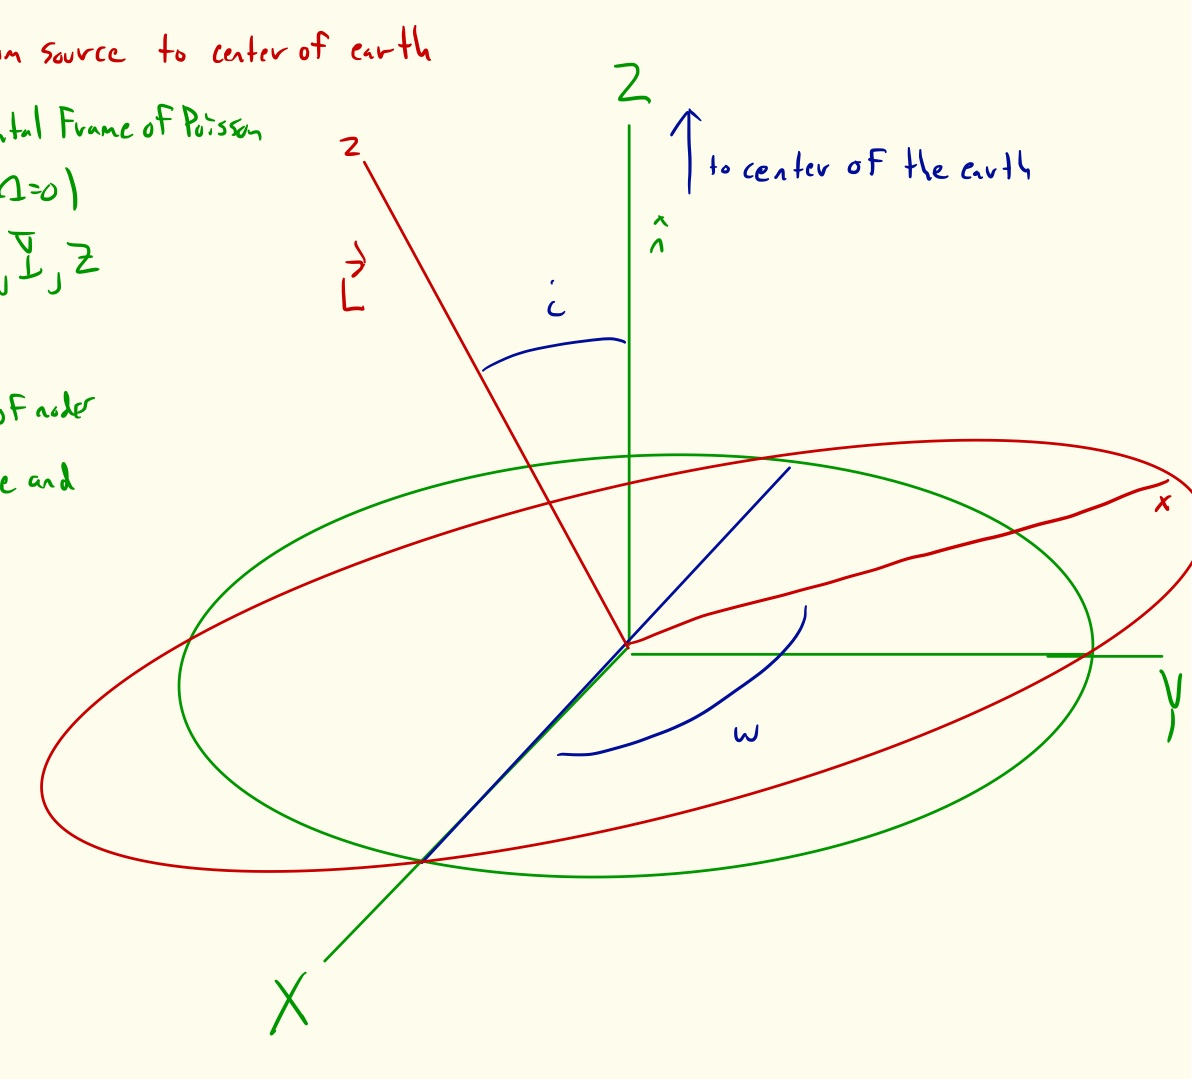
\includegraphics[width =0.45\columnwidth]{sw}
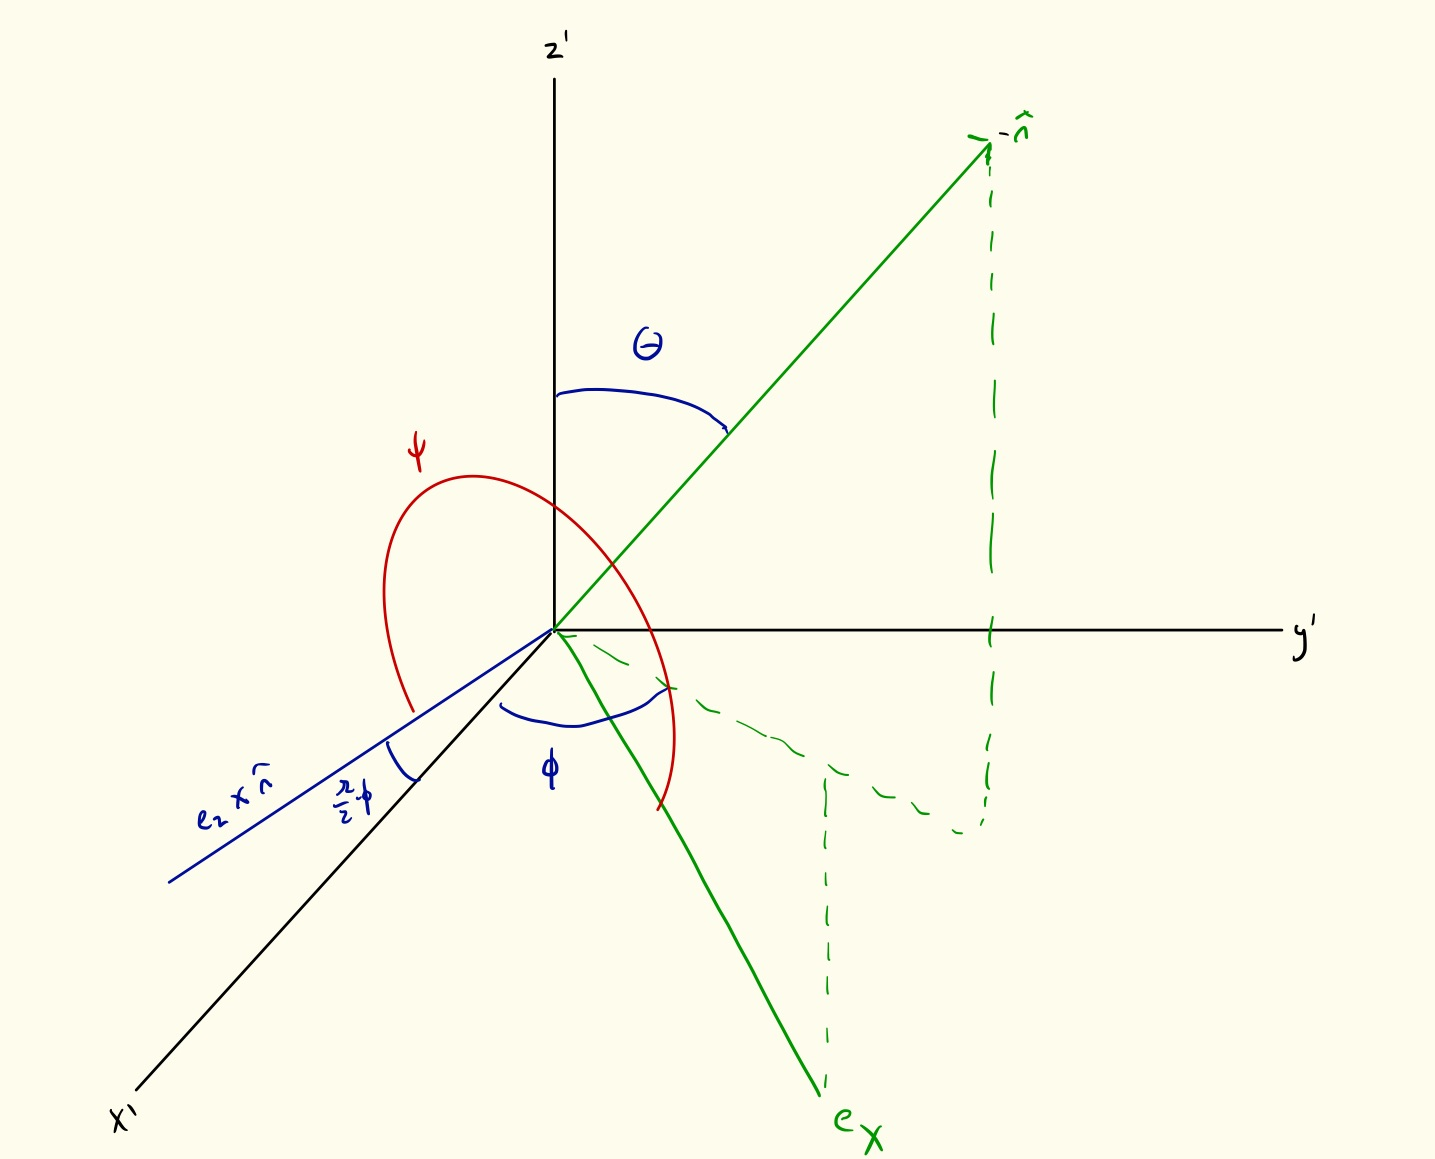
\includegraphics[width =0.5\columnwidth]{we}
\caption{
}
\label{fig:frames}
\end{figure}

The relation between the source frame and the wave frame is shown in the left panel of figure \ref{fig:frames}. The angle between the $z$ and $Z$ axes is $\iota$ and the angle between the $x$ and $X$ axes is $\omega$; however with our conventions $\omega$ is fixed so that $\hat n \cdot \vec e_x=\cos(\pi/2-\iota)=\sin \iota$.

The wave frame coordinates $(X,Y,Z)^T$ of any point can be obtained from the source frame coordinates $(x,y,z)^T$ by a sequence of two rotations
\begin{align}
\begin{bmatrix}
X \\ Y \\ Z
\end{bmatrix}
R_2R_1
\begin{bmatrix}
x \\ y \\ z
\end{bmatrix}
\end{align}
The matrix $R_1$ is a rotation that undoes $\omega$, i.e it rotates by $-\omega$ about $\vec e_z$,
\begin{align}
R_1=
\begin{bmatrix}
\cos(- \omega) & \sin (-\omega) & 0\\
-\sin(-\omega) & \cos(- \omega) & 0 \\ 
0 & 0 & 1
\end{bmatrix}
\end{align}
Performing this rotation aligns $\vec e_x$ with the line of nodes between the plane transverse to $\vec e_Z$ and the xy plane, allowing us to rotate $\vec e_z$ into $\vec e_Z$ by a rotation of $-\iota$ about the new $e_x$ axis, i.e the line of nodes,
\begin{align}
R_2=
\begin{bmatrix}
1 & 0 & 0 \\
0 & \cos (-\iota) & \sin (-\iota) \\ 0 & -\sin (-\iota) &  \cos(-\iota).
\end{bmatrix}
\end{align}

Multiplying the matrices yields the coordinate transformation
\begin{align}
X&=(\cos \omega) x-(\sin \omega) y \nonumber \\
Y& =(\cos \iota) (\sin \omega) x +(\cos \iota \cos\omega)y-(\sin\iota)z \nonumber \\
Z&=(\sin \iota \sin \omega)x +(\sin \iota \cos \omega)y +\cos (\iota) z \label{eq:stoW}
\end{align}

Waveform models typically produce $h_+$ and $h_\times$ in the source frame. To get $h_+$ and $h_\times$ in the wave frame we simply evaluate them in the source frame in the $\hat n$ direction, i.e. with a polar angle of $\iota$ and an azimuthal angle of $0$.

When we discuss gravitational wave detector, we will require a third ``earth'' frame (with the origin at the center of the earth) with cartesian coordinate x', y', and z'. In the earth frame the $\vec e_{z'}$ vector points towards the north pole and the $\vec e_{x'}$ vector points toward the intersection of the prime meridian and the equator. In the earth frame, the source has spherical polar coordinate $\theta =\pi/2 -\delta$ and $\phi=\alpha-GMST$, where $\delta$ is the declination, $\alpha$ is the right ascension, and $GMST$ is the Greenwich mean sidereal time.

The relation between the earth frame and the wave frame is shown in the right panel of fig. \ref{fig:frames}. The polarization angle $\psi$ is defined as the angle from the line of nodes (of the x'y' plane and the XY plane) to the $\hat e_X$ vector, measured counter clockwise around $\hat n$. 

The earth frame coordinates $(x',y',z')^T$ of any point can be obtained from the wave frame coordinates $(X,Y,Z)^T$ by a sequence of three rotations
\begin{align}
\begin{bmatrix}
x' \\ y' \\z'
\end{bmatrix}
=R_3R_2R_1\begin{bmatrix}
X\\ Y \\Z
\end{bmatrix}
\end{align}
The matrix $R_1$ is a rotation that undoes $\psi$, i.e. it rotates by $-\psi$ around $\vec e_Z$:
\begin{align}
R_1=\begin{bmatrix}
\cos (-\psi) & \sin (-\psi) 0 \\
-\sin (-\psi) &\cos (-\psi) 0 \\
0 & 0 &1
\end{bmatrix}
\end{align}
Peforming this rotation aligns the $\vec e_X$ axis with the line of nodes, allowing us to rotate the $Z$ axis into the $z'$ axis with a rotation around the rotated $X$ axis (i.e the line of nodes)
Hence the matrix $R_2$ is a rotation around the line of nodes by $-(\pi-\theta)$:
\begin{align}
R_2=
\begin{bmatrix}
1 &0 & 0 \\
0 &\cos(\theta -\pi) & \sin(\theta-\pi) \\
0 & -\sin(\theta-\pi) & \cos(\theta -\pi)
\end{bmatrix}
\end{align}
Once $R_2$ has aligned the $z'$ axis with the $Z$ axis, we can perform a third rotation around the $z'$ axis by the angle between the line of nodes and the $x'$ axis, which is $\pi/2 -\phi$,
\begin{align}
R_3=
\begin{bmatrix}
\cos (\pi/2-\phi) & \sin(\pi/2-\phi) &0 \\
-\sin (\pi/2-\phi) & \cos(\pi/2-\phi) & 0 \\ 
0 & 0 & 1
\end{bmatrix}
\end{align}

Multiplying these three rotations together shows that the coordinate transformation is
\begin{align}
x'&=[\cos\psi \sin\phi-\sin\psi \cos\theta \cos\phi]X+[-\sin\psi\sin\phi-\cos\psi \cos\theta\cos\phi]Y-\sin\theta \cos\phi Z \nonumber \\
y'&=[-\cos\psi\cos\phi-\sin\psi\cos\theta\sin\phi]X
+[\sin\psi\cos\phi-\cos\psi\cos\theta\sin\phi]Y
-\sin\theta \sin\phi Z \nonumber \\
z'&=\sin\theta \sin\psi X+\sin\theta\cos\psi Y-\cos\theta Z,
\end{align}
which means that the basis vectors are related via
\begin{align}
\vec e_X&=[\cos\psi \sin\phi-\sin\psi \cos\theta \cos\phi]\vec e_{x'}
+[-\cos\psi\cos\phi-\sin\psi\cos\theta\sin\phi]\vec e_{y'}
+\sin\theta \sin\psi\vec e_{z'} \nonumber \\
\vec e_Y&=[-\sin\psi\sin\phi-\cos\psi \cos\theta\cos\phi]\vec e_{x'}
+[\sin\psi\cos\phi-\cos\psi\cos\theta\sin\phi]\vec e_{y'}
+\sin\theta\cos\psi \vec e_{z'} \\
\vec e_{Z}&=-\sin\theta \cos\phi \vec e_{x'}
-\sin\theta \sin\phi \vec e_{y} -\cos\theta e_{z'} \label{eq:wavebasis}
\end{align}
\zach{ZM: The expressions for $e_X$ and $e_Y$ agree with eq.'s A.5a and A.5b of Creighton...Although may want to check again}





\bibliography{QNMModelRefs.bib}

\end{document}